\section{Membuat Button Dengan Blank Page}
Berikut adalah bab bonus untuk mengaetahui cara membuat Button dan menjalankan dengan sebuah link didalamnya, pada bab selanjutnya akan menggunakan halaman yang sama yaitu TEST PAGE.
\begin{enumerate}\begin{figure}
	\item Pertama tama kita membuat blank page terlebih dahulu pilih blank page, lihat pada Gambar 10.1.
	
        \centering
        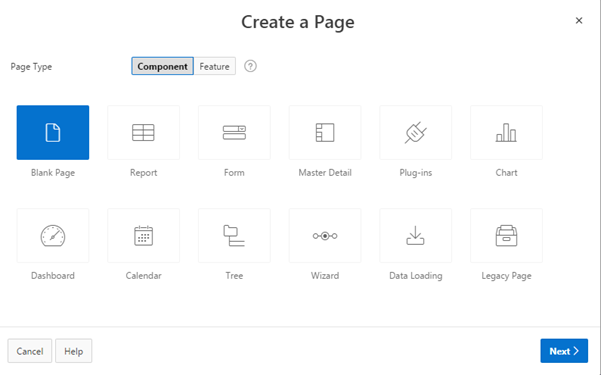
\includegraphics[scale=0.5]{figures/bab10/1.png}
        \caption{\textit{Membuat Blank Page Button}}
        \label{Membuat Blank Page}
    \end{figure}
	\begin{figure}
	\item Kedua beri nama halaman tersebut TEST PAGE, abaikan yang lain lalu klik next, lihat pada Gambar 10.2.
	
        \centering
        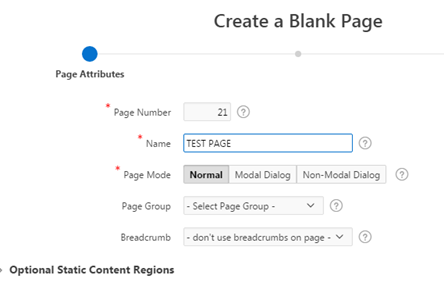
\includegraphics[scale=0.55]{figures/bab10/2.png}
        \caption{\textit{Membuat Blank Page Button 2}}
        \label{Membuat Blank Page 2}
    \end{figure}
	\begin{figure}
	\item Seperti biasa buat navigasi, namun jangan dipilih, kita biarkan default karna akan langsung muncul pada menu navigasi sebelah kiri, lihat pada Gambar 10.3.
	
        \centering
        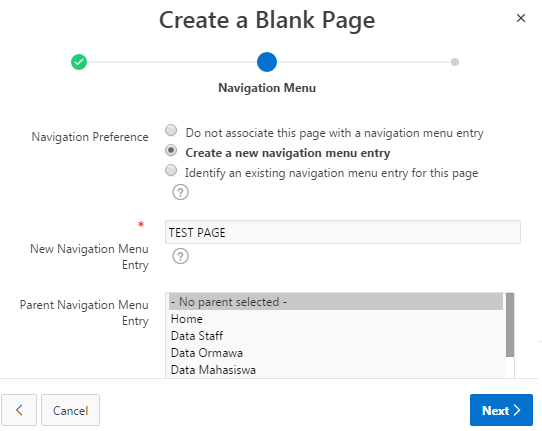
\includegraphics[scale=0.55]{figures/bab10/3.png}
        \caption{\textit{Membuat Blank Page Button 3}}
        \label{Membuat Blank Page 3}
    \end{figure}
    \begin{figure}
	\item Klik finish, lihat pada Gambar 10.4.
	
        \centering
        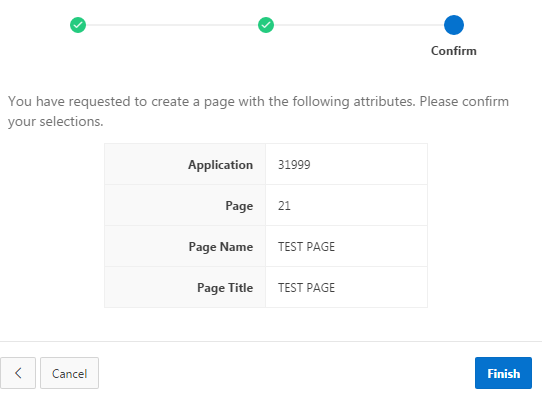
\includegraphics[scale=0.5]{figures/bab10/4.png}
        \caption{\textit{Membuat Blank Page Button 4}}
        \label{Membuat Blank Page 4}
    \end{figure}
	\begin{figure}
	\item Tampilan halaman akan seperti ini, lihat pada Gambar 10.5.
	
        \centering
        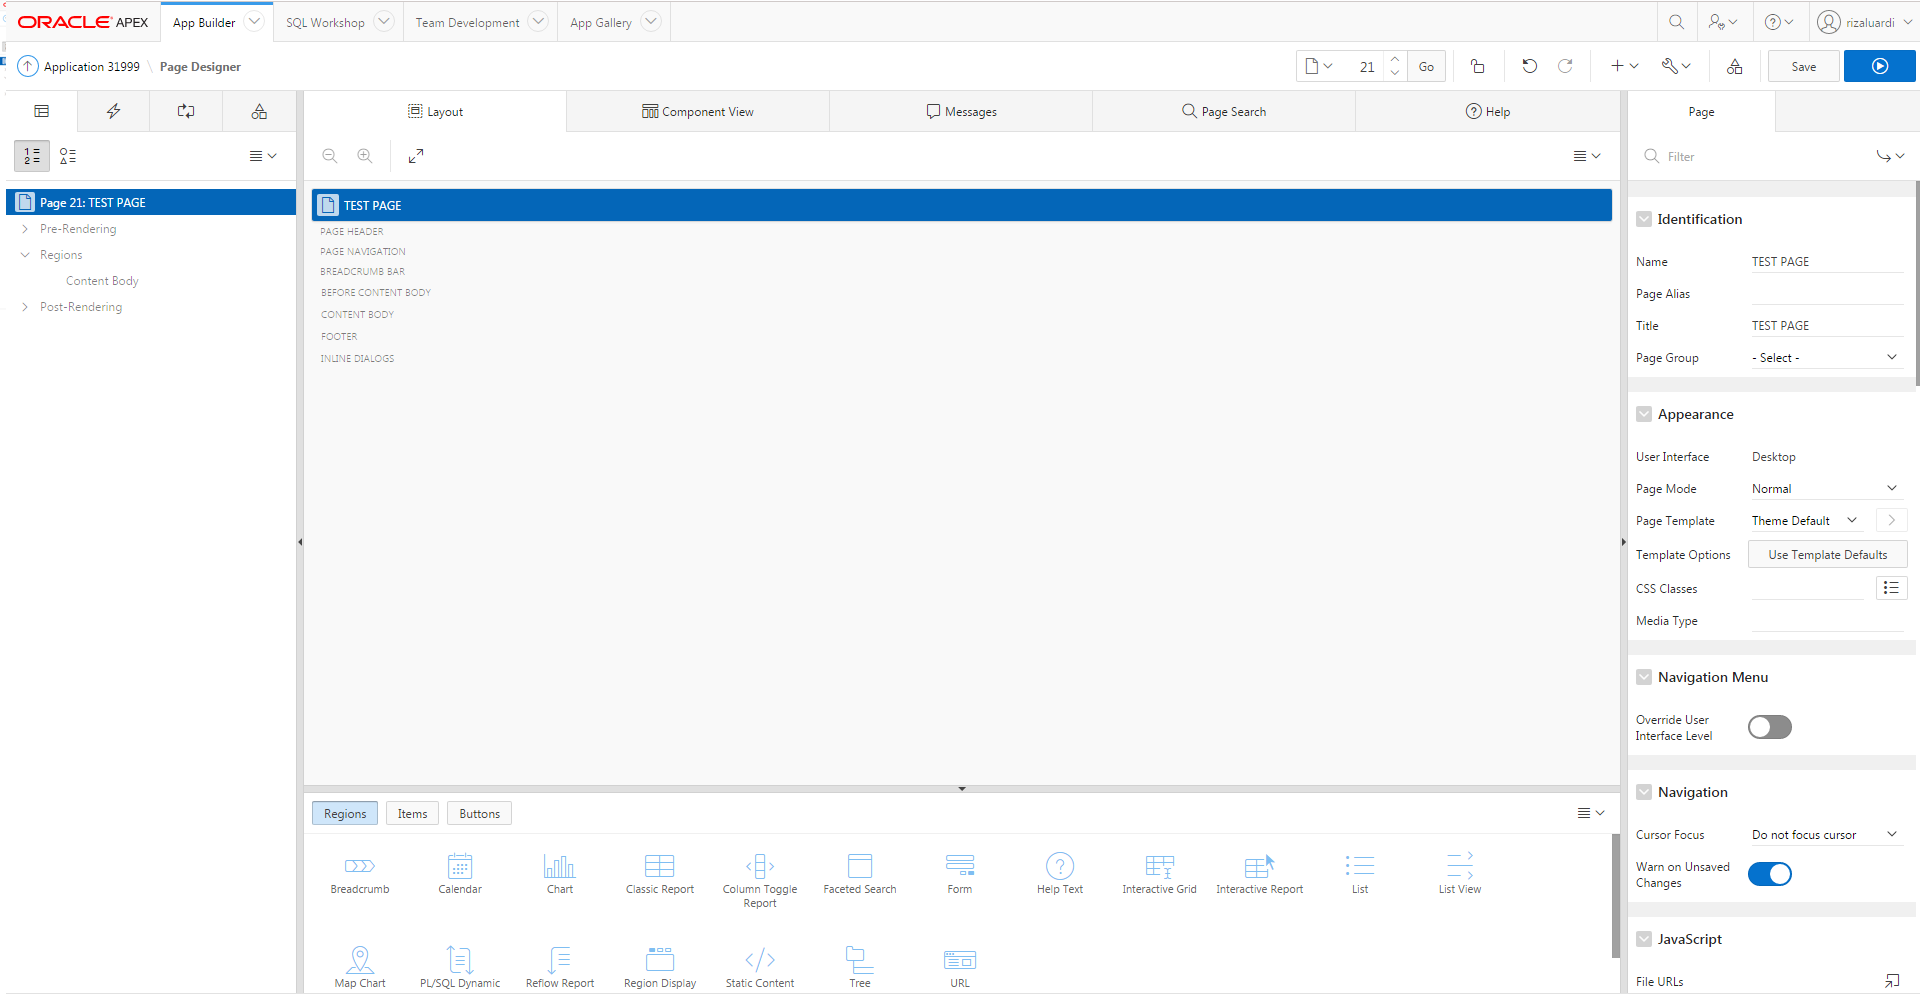
\includegraphics[scale=0.2]{figures/bab10/5.png}
        \caption{\textit{Tampilan Blank Page}}
        \label{}
    \end{figure}
    \begin{figure}
    \item Untuk membuat button pertama kita pilih pda tab regions Breadcumb lalu tarik ke Content Body, lihat pada Gambar 10.6.
	
        \centering
        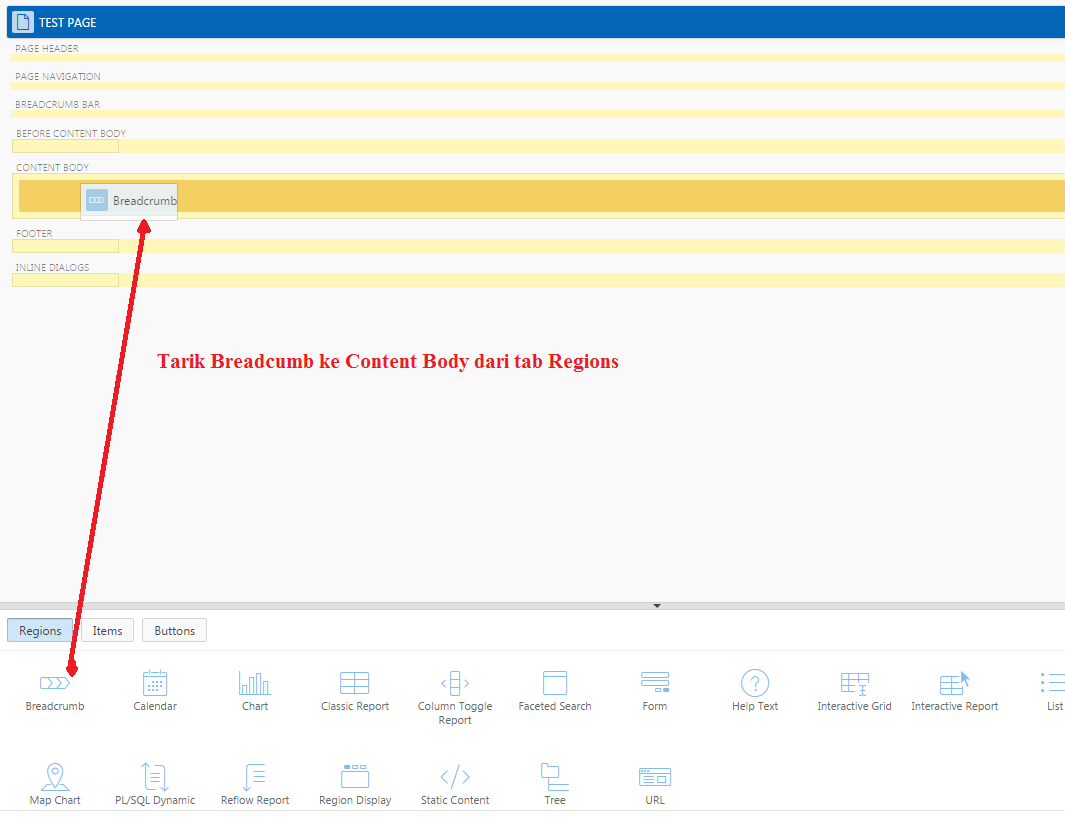
\includegraphics[scale=0.4]{figures/bab10/6.png}
        \caption{\textit{Pilih Breadcumb}}
        \label{Pilih Breadcumb}
    \end{figure}
    
	\begin{figure}
	\item Pada navigasi oracle sebelah kanan terlihat ada Identification dan Source pilih Type dan Breadcumb menjadi Breadcumb, lihat pada Gambar 10.7.
	
        \centering
        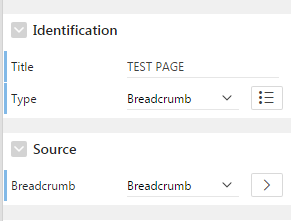
\includegraphics[scale=0.7]{figures/bab10/7.png}
        \caption{\textit{Identification Breadcumb}}
        \label{Identification Breadcumb}
    \end{figure}
	\begin{figure}
	\item pada item button di navigasi bawah ada 6 macam tipe button ada dengan icon,hot icon,text,hot text,text dengan icon,dan text dengan icon hot, lihat pada Gambar 10.8.
	
        \centering
        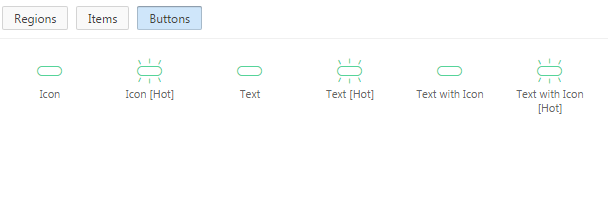
\includegraphics[scale=0.55]{figures/bab10/8.png}
        \caption{\textit{Macam Jenis Icon}}
        \label{Macam Jenis Icon}
    \end{figure}
	\begin{figure}
	\item tarik button text pada item page, lihat pada Gambar 10.9.
	
        \centering
        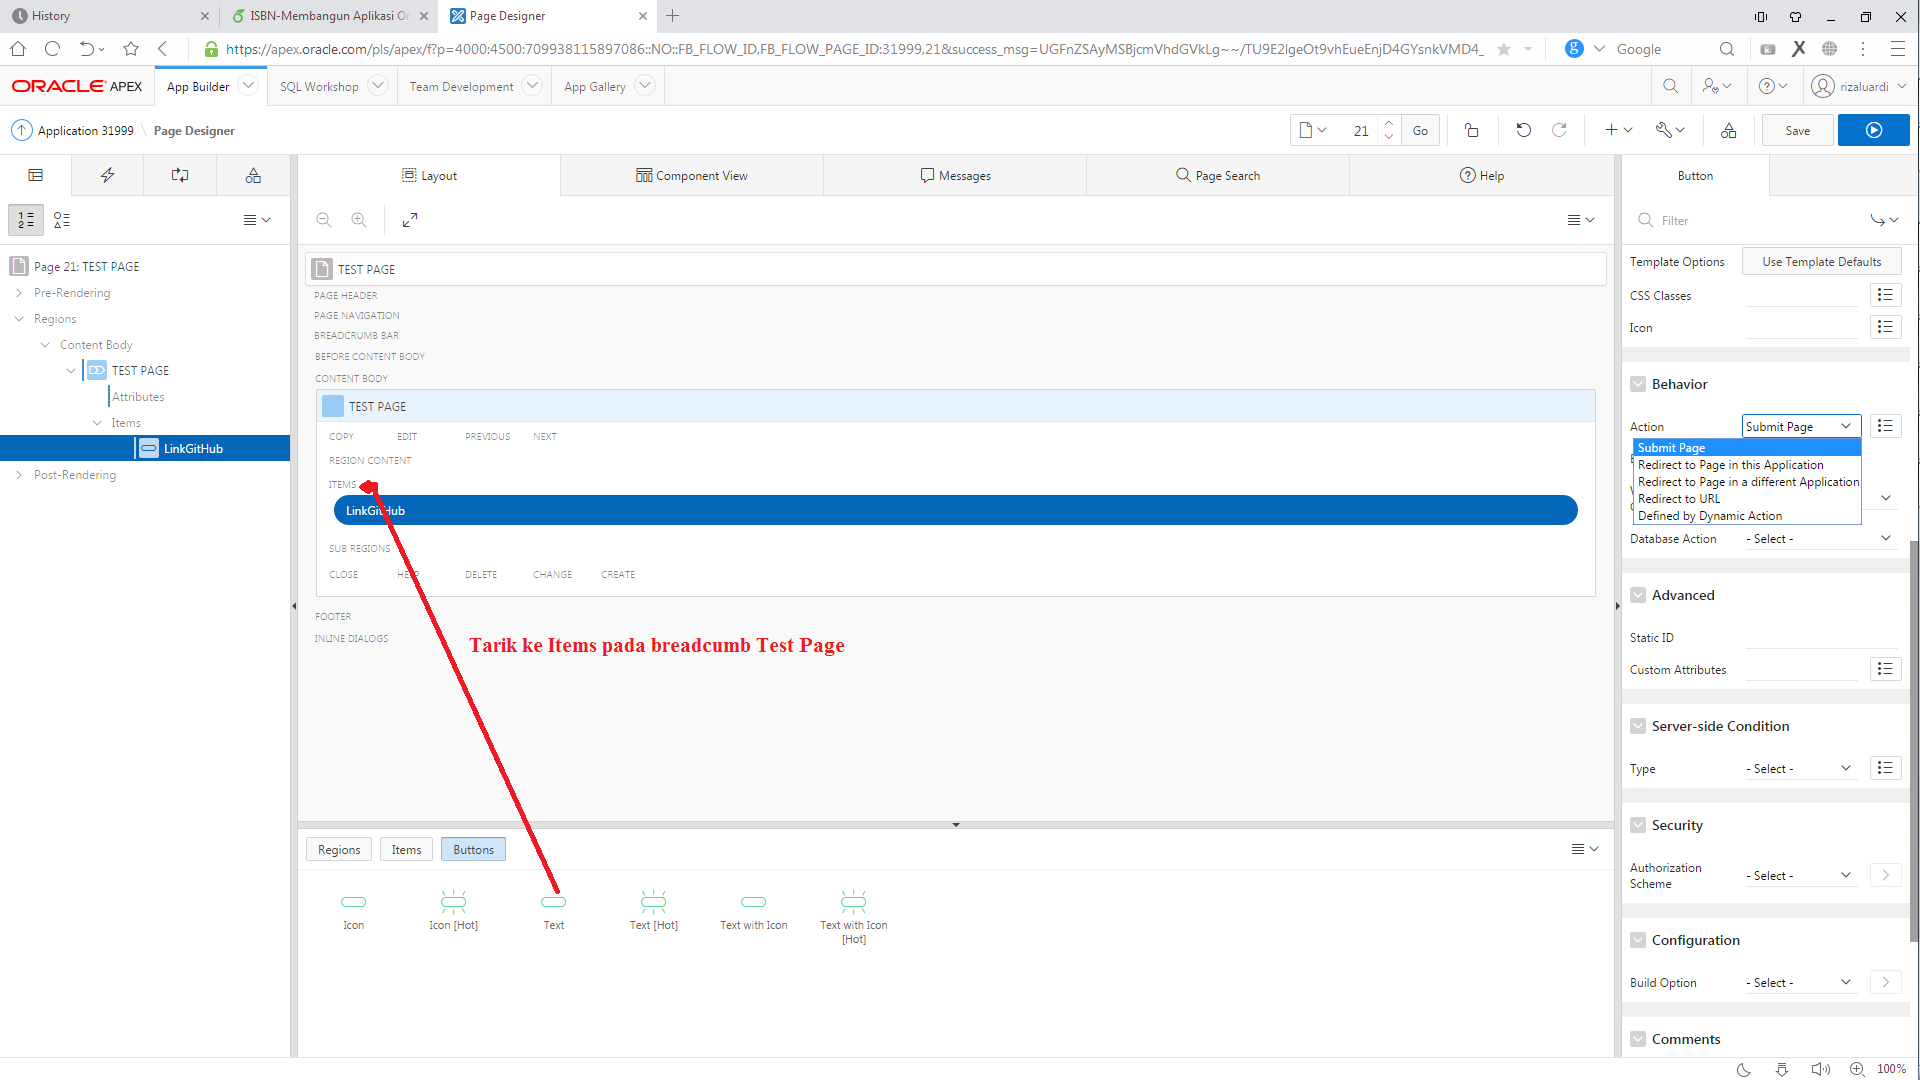
\includegraphics[scale=0.22]{figures/bab10/15.png}
        \caption{\textit{Memasukkan Button pada Breadcumb}}
        \label{Memasukkan Button Pada Breadcumb}
    \end{figure}
	\begin{figure}
	\item Isi Identification dengan Nama, pastikan Button Name tidak diberi spasi atau gunakan Underscore untuk memberi jark antara huruf, beri nama Label untuk agar terlihat pada User Interface Aplikasi, lihat pada Gambar 10.10.
	
        \centering
        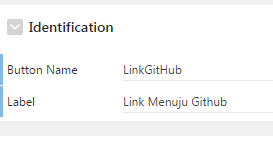
\includegraphics[scale=0.7]{figures/bab10/9.png}
        \caption{\textit{Identification Button}}
        \label{Identification Button}
    \end{figure}
    \begin{figure}
	\item Di bawahnya Identification ada Tab Behavior pilih action menjadi Redirect To Url, lihat pada Gambar 10.11.
	
        \centering
        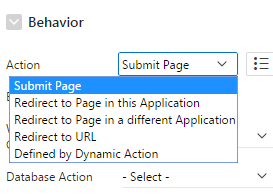
\includegraphics[scale=0.7]{figures/bab10/10.png}
        \caption{\textit{Behavior Button}}
        \label{Behavior Button}
    \end{figure}
    \begin{figure}
	\item klik link target No Link Defined, lihat pada Gambar 10.12.
	
        \centering
        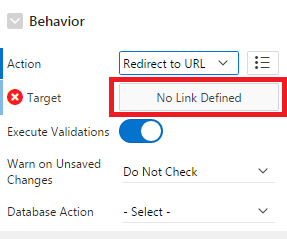
\includegraphics[scale=0.7]{figures/bab10/11.png}
        \caption{\textit{Link Target}}
        \label{Link Target}
    \end{figure}
	\begin{figure}
	\item isikan link target button contoh github.com/rizaluardi lalu klik ok dan save, lihat pada Gambar 10.13.
	
        \centering
        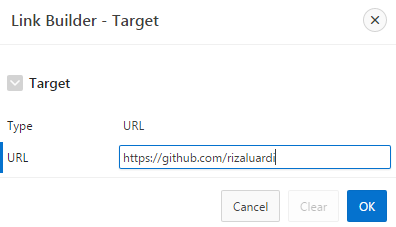
\includegraphics[scale=0.65]{figures/bab10/12.png}
        \caption{\textit{Link Target 2}}
        \label{Link Target 2}
    \end{figure}
	\begin{figure}
	\item hasilnya akan seperti berikut, lihat pada Gambar 10.14.
	
        \centering
        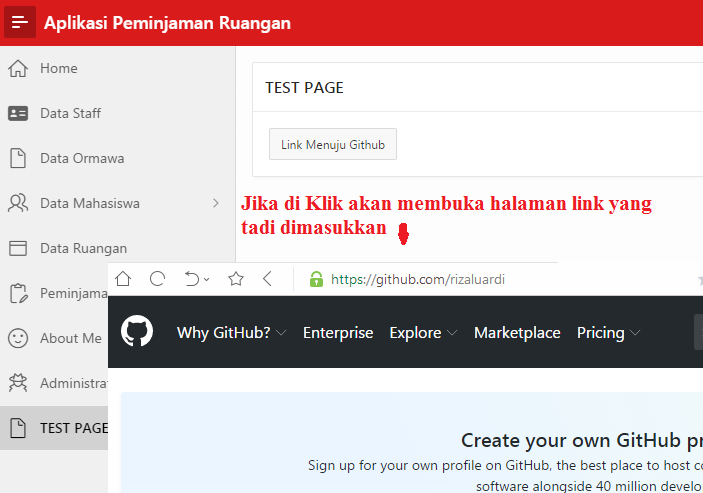
\includegraphics[scale=0.5]{figures/bab10/13.png}
        \caption{\textit{Hasil Button}}
        \label{Hasil Button}
    \end{figure}
	\begin{figure}
	\item anda juga bisa memberi button dengan icon, lihat pada Gambar 10.15.

        \centering
        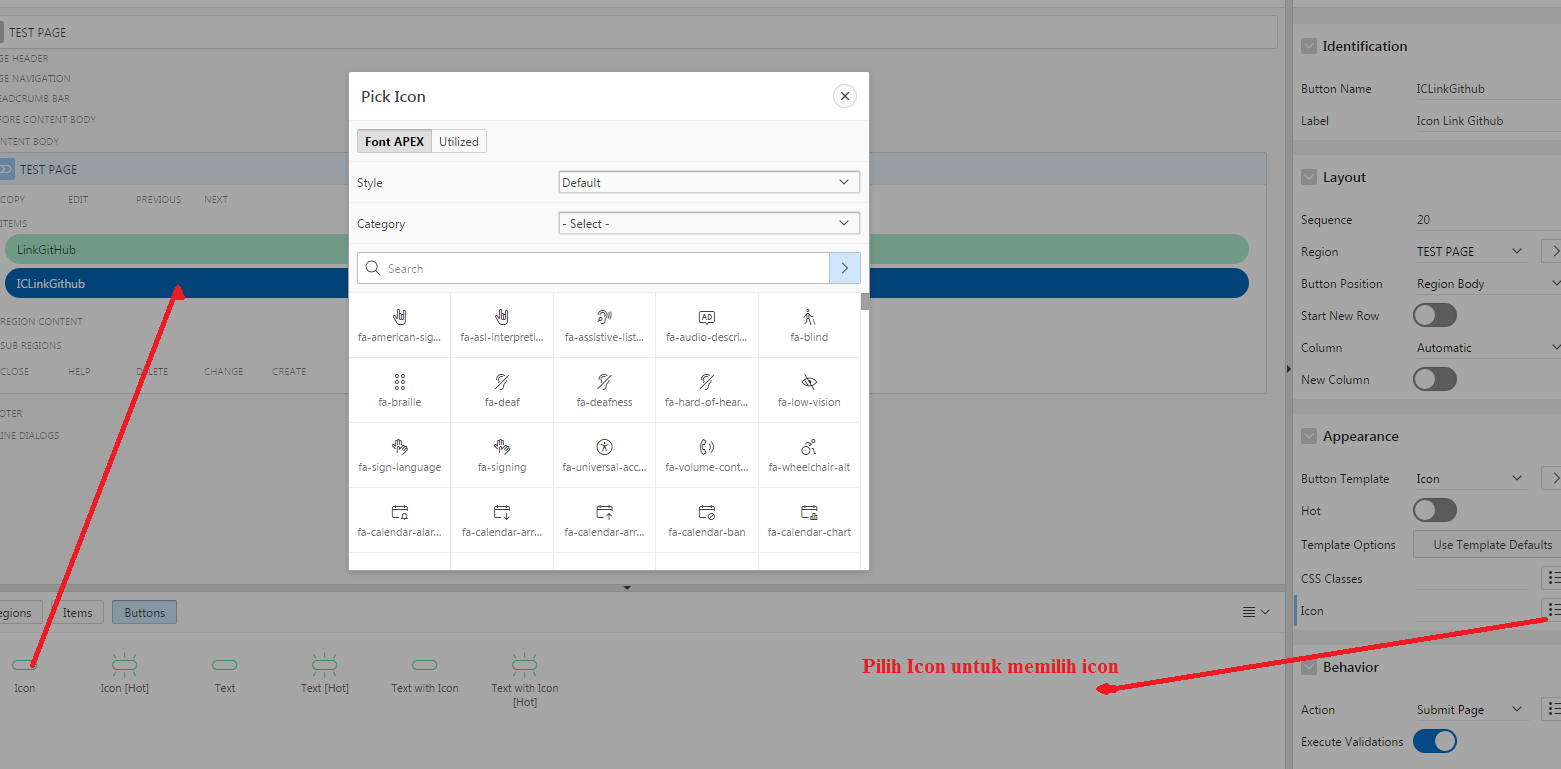
\includegraphics[scale=0.25]{figures/bab10/14.png}
        \caption{\textit{Button Icon}}
        \label{Button Icon}
    \end{figure}

\end{enumerate}

 




